% arara: indent: {overwrite: yes}
\section{Лабораторная 5}

\subsection{Условие}

\textbf{Согласно варианту 10:}
\begin{equation}
	A = \begin{pmatrix}
			1.2 & 0.1 & -0.3 \\
			-0.3 & 0.9 & -0.2 \\
			0.4 & 0.5 & 1.0 \\
		\end{pmatrix},
	f = \begin{pmatrix}
			2 \\
			3 \\
			3
		\end{pmatrix}.
\end{equation}

Решить систему линейных уравнений, используя метод Монте-Карло.

\begin{enumerate}
	\item Решить систему линейных алгебраических уравнений $Ax = f$ методом Монте-Карло;
	\item Сравнить с решением данного уравнения, полученным в произвольном математическом пакете;
	\item Построить график зависимости точности решения от длины цепи Маркова и числа смоделированных цепей Маркова.
\end{enumerate}

\subsection{Теория}
\subsubsection{Метод Монте-Карло для решения СЛАУ}

Для необходимо привести СЛАУ к виду
\begin{equation}
x = Ax + f.
\end{equation}

Предположим, что наибольшее по модулю характеристическое число матрицы $A$ меньше единицы, так что сходиться метод последовательных приближений:
\begin{equation}
x^{(k)} = Ax^{(k-1)} + f, k = 1,2,\ldots
\end{equation}

Достаточным условием для того, чтобы все характеристические числа матрицы $A$ лежали внутри единичного круга на комплексной плоскости, то есть $|\lambda_{i}| < 1, i = \overline{1, n}$ может служить одно неравенств:
\begin{equation}
	\begin{array}{l}
		\sum\limits_{i,j=1}^{n}a_{ij}^{2} < 1\\
		\max\limits_{1 \leqslant i \leqslant n}\sum\limits_{j=1}^{m}|a_{ij}|<1
	\end{array}
\end{equation}

Пусть размерность вектора $x$ равна $n$. Для нахождения компоненты $x_{i}$ вектора $x$ определим вектор:
\begin{equation}
	h=\begin{cases}
		h_{j}=0, j \neq i \\
		h_{i}=1, j = \overline{1,n}
	\end{cases}.
\end{equation}

Моделирование цепи Маркова выглядит следующим образом:
\begin{equation}
i_{0} \rightarrow i_{1} \rightarrow \ldots \rightarrow i_{N-1}, i_{k} \in {\overline{1,n}}.
\end{equation}

Вектор вероятностей начальных состояний цепи Маркова:
\begin{equation}
\pi = \left\lbrace\pi_{i} = \frac{1}{n}, i = \overline{1,n} \right\rbrace.
\end{equation}

Матрица переходных вероятностей имеет вид:
\begin{equation}
P = \left\lbrace P_{ij} = \frac{1}{n}, i,j = \overline{1,n} \right\rbrace.
\end{equation}

Каждому состоянию цепи Маркова приписываем веса, которые вычисляются по формулам:
\begin{equation}
\begin{array}{l}
	Q_{i_{0}}=g_{i_{0}}=\begin{cases}
							\frac{h_{i_{0}}}{\pi_{i_{0}}}, \pi_{i_{0}} > 0, \\
							0, \pi_{i_{0}} = 0
						\end{cases}\\
	\ldots \\
	Q_{i_{k}}=Q_{i_{k-1}}g_{i_{k-1}}=\begin{cases}
										\frac{a_{i_{k-1}i_{k}}}{p_{i_{k-1}i_{k}}}, p_{i_{k-1}i_{k}} > 0,\\
										0, p_{i_{k-1}i_{k}} = 0
									 \end{cases}
\end{array}.
\end{equation}

\paragraph{Алгоритм моделирования:}\
\

Моделировать СВ $\xi_{N}$ будем по формуле:
\begin{equation}
\xi_{N}^{(l)}=\sum\limits_{n=0}^{N}=Q_{i_{n}}f_{i_{n}}
\end{equation}

где $l=\overline{1,L}$ - номер реализации цепи Маркова. Тогда приближённое решение вычисляется по формуле:
\begin{equation}
x_{i} \approx \frac{1}{L}\sum\limits_{l=1}^{L}\xi_{N}^{(l)}, i = \overline{1,n}.
\end{equation}

\subsection{Код программы}

\lstinputlisting[language=Python]{./lab_5/lab5.py}

\subsection{Результат выполнения}

\begin{figure}[H]
	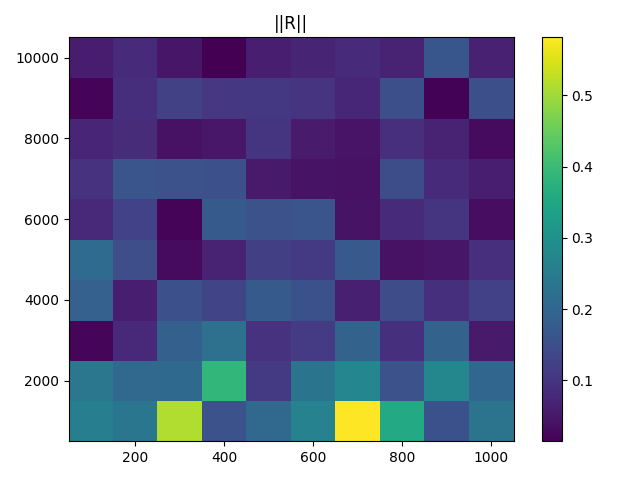
\includegraphics[width=\textwidth]{results_lab_5.png}
	\label{fig:results_lab_5}
	\caption{График зависимости точности решения от длины цепи маркова - ось $Ox$ и числа цепей Маркова - ось $Oy$.}
\end{figure}
